\documentclass[../main.tex]{subfiles}
\begin{document}

\chapter{Überblick}
\label{overview}
\pagenumbering{arabic}
  Virtualisierung entwickelte sich in den letzten Jahren zu einem allgegenwärtigen Thema in der IT-Industrie. Unter ihr versteht man die Nachahmung und Abstraktion von physischen Resourcen, z.B. der CPU oder des Speichers, die in einem virtuellen Kontext von Softwareprogrammen genutzt wird.

  Die Vorteile von Virtualisierung umfassen Hardwareunabhängigkeit, Verfügbarkeit, Isolierung und Sicherheit, welche die Erfolgsgrundlage der Virtualisierung in heutigen Cloud-Infrastrukturen bilden \cite[S.1]{containerVirtPerformance}. Vor allem in Rechenzentren bieten sich Virtualisierungen an, um die Serverressourcen effizienter zu nutzen \cite[S.1]{dockerSec1}. Letztendlich haben es Virtualisierungen ermöglicht, Serverressourcen in der Form von \glspl{Cloud} wie z.B. den \emph{Amazon Web Services}\cite{amazonWebServices} und auf Basis eines Subskriptionsmodells nutzen zu können \cite[S.1]{dockerSec1}.

  Heutzutage existieren mehrere serverseitige Virtualisierungstechniken, wovon die Hypervisor-gestützen Methoden mit den etablierten Vertretern \emph{Xen}\cite{xen}, \emph{KVM}\cite{kvm}, \emph{VMware ESXi}\cite{vmwareESXi} und \emph{Hyper-V}\cite{hyperv} die meistverbreitesten sind \cite[S.2]{containerVirtPerformance}. Der alternativen containerbasierten Virtualisierung ist es erst mit Docker im Jahr 2013 zum Durchbruch gekommen

  % TODO: WEITERMACHEN HIER

  Mit dem Release von Docker im März 2013 \cite{githubDockerChangelog}, erlebte die Virtualisierung auf Containerbasis einen Aufschwung. Wie die Google Trends in \fig \ref{fig:overview_googleTrends} zeigen, stieg das Interesse an Docker seit dessen Release kontinuierlich an, während das Suchwort \glqq{}virtualization\grqq{} im Jahr 2010 seinen Höhepunkt hatte und seitdem an Popularität verlor. Auch das Interesse an der Containertechnologie \emph{LXC}, aus der Docker entstand, bleibt weit hinter der von Docker zurück \cite{googleTrends}.

  \begin{figure}[h]
      \centering
      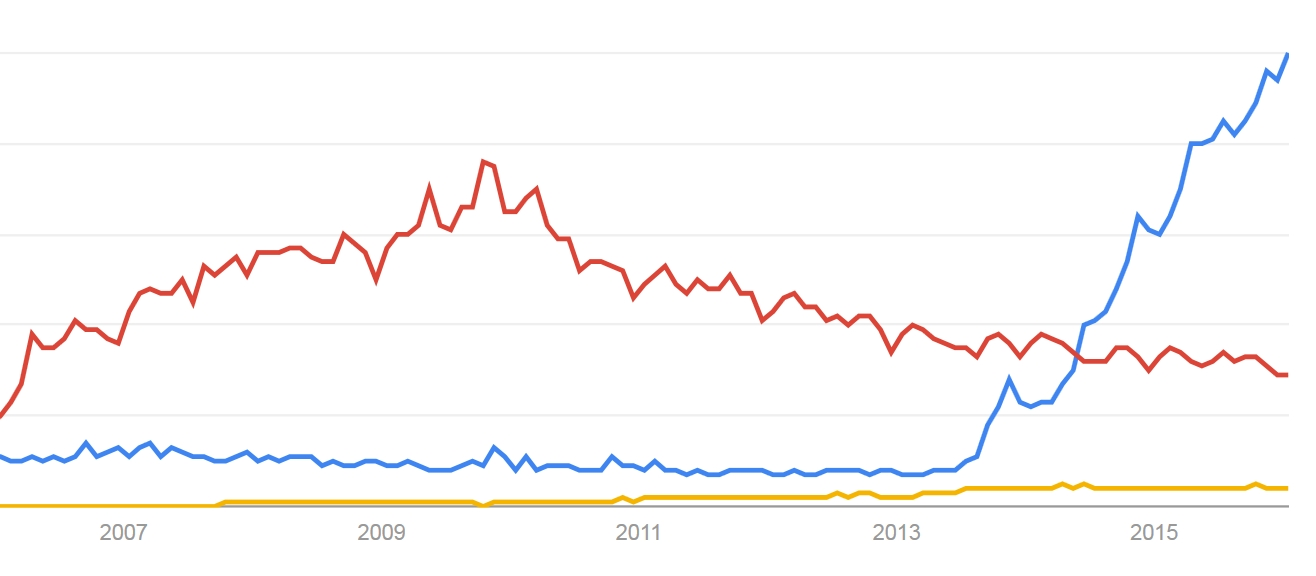
\includegraphics[width=1.0\textwidth]{./images/googletrend_dockerVirtualizationLXC.jpg}
      \caption{Google Trends der Suchbegriffe \glqq{}Virtualization\grqq{} (rot), \glqq{}Docker\grqq{} (blau) und \glqq{}LXC\grqq{} (gelb) von Januar 2006 bis Januar 2016\cite{googleTrends}.}
      \label{fig:overview_googleTrends}
  \end{figure}

  Obwohl das Konzept von Containern bereits im Jahr 2000 als \emph{Jails} in dem Betriebssystem \emph{FreeBSD} und seit 2004 als \emph{Zones} unter \emph{Solaris} verwendet wurde \cite{zonesReleasenotes}\cite{jailsReleasenotes}, gelang keiner dieser Technologien vor Docker der medienwirksame Durchbruch. Wie Docker den bis 2013 vorherrschenden Ruf von Containertechnologien, dass Container noch nicht ausgereift seien \cite[S.8]{containerVirtPerformance}, nachhaltig verändern konnte, ist in der Einführung zu Docker in Kapitel \ref{dockerIntro} beschreiben.

  Heute sind Container in vielen Szenarien, v.a. skalierbaren Infrastrukturen, trotz intrinsischer Sicherheitsschwächen gegenüber Hypervisor-gestützten Virtualisierungsarten beliebt. Vor allem \glspl{MultiTenantService} werden gerne mit Docker umgesetzt \cite[S.6]{dockerBook}\cite{dockerUnderstandingDocker}.

  % https://www.airpair.com/firebase/posts/yatodo-guide
  % https://www.airpair.com/docker/posts/8-proven-real-world-ways-to-use-docker#7-multi-tenancy


  \section{Struktur der Arbeit}
    Die zwei prominentesten Virtualisierungstechniken, Hypervisor-basierte (Sektion \ref{introVirtHypervisor}) und Container-basierte (Sektion \ref{introVirtContainer}) Virtualisierung, werden im Grundlagenkapitel \ref{introVirt} gegenübergestellt.

    In diesem Kapitel wird nur die für diese Arbeit relevante Techniken der systembasierten Virtualisierung beschrieben, also solche, in denen Betriebssysteme ablaufen. Die Anwendungs-, Storage- oder Netzwerkvirtualisierung wird nicht behandelt.

    % folgende 2 Absätze in "Struktur der Arbeit"?
    Die Themen Virtualisierung, Sicherheit in der IT sowie Docker sind sehr weitreichende Themengebiete. Um in den einleitenden Kapiteln nicht ausführlich zu werden, sind Eckdaten einiger Begriffe im angehängten Glossar zusammengefasst.

    In der Arbeit vorkommende Produkt-, Technologie- oder Unternehmensnamen sind durchgehend \emph{kursiv} gedruckt. Eine Ausnahme bildet Docker, in der die reguläre Schreibweise für die Plattform Docker vorgesehen ist, während die kursive Variante das Unternehmen \emph{Docker} meint.

\end{document}
